\documentclass[letterpaper, onecolumn, 11pt]{report}
\usepackage[utf8]{inputenc}
\usepackage[spanish]{babel}
\usepackage{amsmath}
\usepackage{graphicx}
\usepackage{hyperref}
\usepackage{marginnote}

\renewcommand*{\marginnotevadjust}{-0.1cm}
\renewcommand*{\marginfont}{\footnotesize}
\usepackage[right=4.5cm,left=2cm,top=3cm,bottom=3.0cm]{geometry}

\hypersetup{colorlinks=true, linkcolor=blue}
\begin{document}
\sffamily
\title{\Huge\textbf{{Electromagnetismo}}}
\author{Diez B. Borja}
\maketitle
\tableofcontents
\chapter{Potencial eléctrico }
Cuando una partícula con carga se mueve en un campo eléctrico, el campo ejerce una fuerza que efectúa \textit{trabajo} sobre la partícula. Este trabajo siempre se puede expresar en términos de la energía potencial eléctrica\footnote{O simplemente \textit{potencial eléctrico} o \textit{potencial}}. Una diferencia de potencial entre un punto y otro reciba el nombre de \textit{voltaje}.

\section{Energía potencial eléctrica}
Cuando una fuerza $\vec{F}$ actúa sobre una partícula que se mueve de un punto $a$ a un punto $b$, el trabajo $W_{a\to b}$ efectuado por la fuerza está dado por la siguiente \textit{integral de línea}:

\begin{equation}\label{23.1}\marginnote{Trabajo realizado por una fuerza}
W_{a\to b}=\int_a^b\vec{F}\cdot d\vec{l}=\int_a^bF\cos\phi dl
\end{equation}

donde $d\vec{l}$ es un desplazamiento infinitisimal a lo largo de la trayectoria de la partícula, y $\phi$ es el ángulo entre $\vec{F}$ y $d\vec{l}$ 	en cada punto de la trayectoria.

Si la fuerza $\vec{F}$ es \textit{conservativa}, el trabajo realizado por esta siempre se puedo expresar en términos de una \textbf{energía potencial} $U$. Cuando la partícula se mueve de un punto donde la energía potencial es $U_a$ a otro donde es $U_b$, el cambio de energía potencial es $\Delta U=U_b-U_a$, y el trabajo $W_{a\to b}$ que realiza la fuerza es

\begin{equation}\label{23.2}\marginnote{Trabajo efectuado por una fuerza conservativa}
\boxed{W_{a\to b}=U_a-U_b=-(U_b-U_a)=-\Delta U}
\end{equation}

En tercer lugar, el teorema del trabajo y la energía establece que el cambio en la energía cinética $\Delta K=K_b+K_a$ durante cualquier desplazamiento es igual al trabajo \textit{total} realizado sobre la partícula. Si el único trabajo efectuado sobre la partícula lo realizan fuerzas conservativas, entonces la ecuación \ref{23.2} da el trabajo total, y $K_b-K_a=-(U_b-U_a)$. Es decir, 

\begin{equation}\label{23.3}
K_a+U_a=K_b+U_b
\end{equation}

Es decir, en estas circunstancias, la energía mecánica total (cinética más potencial) se
\textit{conserva}.

\subsection{Energía potencial eléctrica de un campo uniforme}
\begin{figure}[h]
\centering
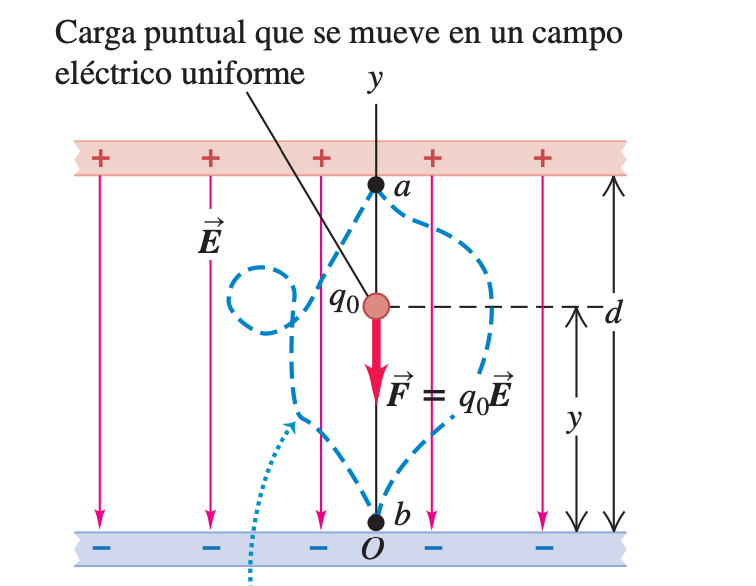
\includegraphics[scale=0.5]{fig/energia_potencial}
\caption{Trabajo realizado sobre una carga puntual que se mueve en un campo eléctrico uniforme. El trabajo realizado por la fuerza eléctrica es el mismo para cualquier trayectoria de $a$ a $b$: $W_{a\to b}=-\Delta U=q_0Ed$} 
\label{fig:energia_potencial}
\end{figure}

En la figura \ref{fig:energia_potencial} un par de placas metálicas paralelas con carga generan un campo eléctrico uniforme descendente y con magnitud $E$. El campo ejerce una fuerza hacia abajo con magnitud $F=q_0E$ sobre una carga de prueba positiva $q_0$. A medida que la carga se mueve hacia abajo una distancia $d$ del punto $a$ al punto $b$, la fuerza sobre la carga de prueba es constante e independiente de su localización. Por lo tanto, el trabajo realizado por el campo eléctrico es 

\begin{equation}\label{23.4}
W_{a\to b}=Fd=q_0Ed
\end{equation}

Este trabajo es positivo, toda vez que la fuerza está en la misma dirección que el desplazamiento neto de la carga de prueba. Este trabajo puede representarse con una función de \textbf{energía potencial} $U$, que para la fuerza eléctrica está dada por

\begin{equation}\label{23.5}
U=q_0Ey
\end{equation}

Cuando la carga de prueba se mueve de la altura $y_a$ a la altura $y_b$, el trabajo realizado sobre la carga por el campo está dado por

\begin{equation}\label{23.6}
W_{a\to b}=-\Delta U=-(U_b-U_a)=-(q_0Ey_b-q_0Ey_a)=q_0E(y_a-y_b)
\end{equation}

\subsection{Energía potencial entre dos cargas puntuales}
El concepto de energía potencial se puede aplicar a una carga puntual en \textit{cualquier} campo eléctrico generado por una distribución de carga estática. 
Cualquier distribución de carga se representa como un conjunto de cargas puntuales. Por consiguiente, es útil calcular el trabajo realizado sobre una carga de prueba $q_0$ que se mueve en el campo eléctrico ocasionado por una sola carga puntual estacionaria $q$.

En primer lugar se considerará un desplazamiento a lo largo de una línea radial, del punto $a$ al punto $b$. La fuerza sobre $q_0$ está dada por la ley de Coulomb, y su componente radial es

\begin{equation}\label{23.7}
F_r=\frac{1}{4\pi\epsilon_0}\frac{qq_0}{r^2}
\end{equation}

Si $q$ y $q_0$ tienen el mismo signo, la fuerza es de repulsión y $F_r$ es positiva; en caso contrario la fuerza es de atracción y $F_r$ es negativa. La fuerza \textit{no} es constante durante el desplazamiento, y se tiene que integrar para obtener el trabajo $W_{a\to b}$ que realiza esta fuerza sobre $q_0$ a medida que $q_0$ se mueve de $a$ a $b$

\begin{equation}\label{23.8}
W_{a\to b}=\int_{r_a}^{r_b}F_rdr=\int_{r_a}^{r_b}\frac{1}{4\pi\epsilon_0}\frac{qq_0}{r^2}dr=\frac{qq_0}{4\pi\epsilon_0}\left(\frac{1}{r_a}-\frac{1}{r_b}\right)
\end{equation}

El trabajo es el mismo para todas las trayectorias posibles entre $a$ y $b$. La fuerza sobre $q_0$ es \textit{conservativa}.\\
Se ve que las ecuaciones \ref{23.2} y \ref{23.8} son cosistentes si se define $qq_0/4\pi\epsilon_0r_a$ como la energia potencial $U_a$ cuando $q_0$ está en el punto $a$, a una distancia $r_a$ de $q$, y se define $qq_0/4\pi\epsilon_0r_b$ como la energía potencial $U_b$ cuando $q_0$ está en el punto $b$, a una distancia $r_b$ de $q$. De esta forma, la energía potencial $U$ cuando la carga de prueba $q_0$ está a cualquier distancia $r$ de la carga $q$ es

\begin{equation}\label{23.9.e_potencial}\marginnote{E. potencial eléctrica de dos cargas $q$ y $q_0$}
\boxed{U=\frac{1}{4\pi\epsilon_0}\frac{qq_0}{r}}
\end{equation}

\textbf{Obervación:} De las ecuaciones \ref{23.9.e_potencial} y \ref{23.7} notamos que tienen similitud. La energía potencial $U$ es proporcional a $1/r$, mientras que la componente de la fuerza $F_r$ es proporcional a $1/r^2$.\\
La energía potencial siempre se define en relación con algún punto de referencia donde $U=0$. En la ecuación \ref{23.9.e_potencial}, $U$ es igual a cero cuando $q$ y $q_0$ están infinitamente alejadas y $r=\infty$. Por lo tanto, \textbf{$U$ representa el trabajo que realizaría el campo de $q$ sobre la carga de prueba $q_0$ si esta última se desplazara de una distancia inicial $r$ al infinito}. La energía potencial $U$ es una propiedad \textit{compartida} de las dos cargas $q$ y $q_0$; es una consecuencia de la \textit{interacción} entre dos cuerpos.

La ley de Gauss dice que el campo eléctrico fuera de cualquier distribución de carga esféricamente simétrica es la misma que habría si toda la carga estuviera en el centro.

\subsection{Energía potencial eléctrica con varias cargas putuales}

\begin{figure}[h]
\centering
\caption{La energía potencial asociada con la carga $q_0$ en el punto a depende de las otras cargas $q_1, q_2$ y $q_3$ y de sus distancias $r_1, r_2$ y $r_3$ desde el punto $a$.}
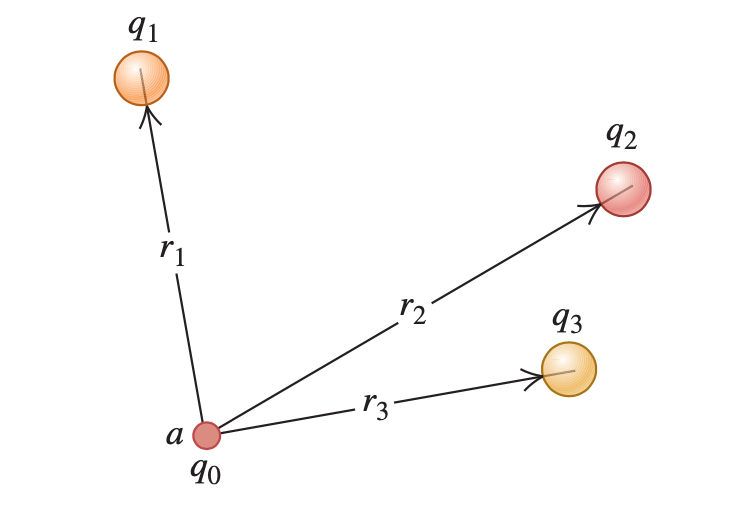
\includegraphics[scale=0.4]{fig/e_potencial_varias}
\label{fig:e_potencial_varias}
\end{figure}

Suponga que el campo eléctrico $\vec{E}$ en el que se desplaza la carga $q_0$ se debe a varias cargas puntuales $q_1, q_2, q_3$, . . . a distancias $r_1, r_2, r_3$, . . . de $q_0$. . El campo eléctrico total en cada punto es la \textit{suma vectorial} de los campos debidos a las cargas individuales, y el trabajo total realizado sobre $q_0$ durante cualquier desplazamiento es la suma de las contribuciones de las cargas individuales. De la ecuación \ref{23.9.e_potencial} se concluye que la energía potencial asociada con la carga de prueba $q_0$ en el punto a en la figura \ref{fig:e_potencial_varias} es la suma \textit{algebraica} (no la suma vectorial).

\begin{equation}\label{23.10}\marginnote{Carga puntual $q_0$ y conjunto de cargas $q_i$}
\boxed{U=\frac{q_0}{4\pi\epsilon_0}\left(\frac{q_1}{r_1}+\frac{q_2}{r_2}+\frac{q_3}{r_3}+\cdots \right)=\frac{q_0}{4\pi\epsilon_0}\sum_{i}\frac{q_i}{r_i}}
\end{equation}

El trabajo efectuado sobre la carga $q_0$ cuando se desplaza de $a$ a $b$ a lo largo de cualquier trayectoria es igual a la diferencia $U_a-U_b$ entre las energías potenciales cuando $q_0$ está en $a$ y en $b$.

Se puede representar \textit{cualquier} distribución de carga como un conjunto de cargas puntuales, por lo que la ecuación \ref{23.10} muestra que \textbf{para todo campo eléctrico debido a una distribución de carga estática, la fuerza ejercida por ese campo es conservativa.}

Las ecuaciones \ref{23.9.e_potencial} y \ref{23.10} definen que $U$ es igual a cero cuando todas las distancias $r_1, r_2, . . .$ son infinitas, es decir, cuando la carga de prueba $q_0$ está muy lejos de todas las cargas que producen el campo.

\subsubsection{Interpretación de la energía potencial eléctrica}
Definimos la energía potencial eléctrica en términos del trabajo realizado por el campo eléctrico sobre una partícula con carga que se mueve en el campo. Cuando una partícula se desplaza del punto $a$ al punto $b$, el trabajo que realiza sobre ella el campo eléctrico es $W_{a\to b}=U_a-U_b$. Por lo tanto, la diferencia de energía potencial $U_a-U_b$ es igual al \textit{trabajo que efectúa la fuerza eléctrica cuando la partícula se desplaza de $a$ a $b$}. Cuando $U_a$ es mayor que $U_b$ el campo realiza trabajo positivo sobre la partícula conforme “cae” de un punto de mayor energía potencial ($a$) a otro con menor energía potencial ($b$).

Un punto de vista alternativo pero equivalente es considerar cuánto trabajo se hubiera tenido que hacer para “subir” la partícula desde un punto $b$, en el que la energía potencial es $U_b$, hasta un punto $a$ en el que la energía potencial tiene un valor mayor $U_a$ (por ejemplo, al empujar dos cargas positivas para acercarlas). Para mover la partícula lentamente (de manera que no se le imparta ninguna energía cinética), es necesario ejercer una fuerza externa adicional $F_{ext}$ que es igual y opuesta a la fuerza del campo eléctrico y realiza un trabajo positivo. La diferencia de energía potencial $U_a-U_b$ se define entonces como el trabajo que debe efectuar una fuerza externa para desplazar la partícula lentamente desde $b$ hasta $a$ en contra de la fuerza eléctrica.

\section{Potencial eléctrico}
El \textbf{potencial} es \textit{la energía potencial por unidad de carga}. Se define el potencial $V$ en cualquier punto en el campo eléctrico como la energía potencial $U$ \textit{por unidad de carga} asociada con una carga de prueba $q_0$ en ese punto:

\begin{equation}\label{23.12}
V=\frac{U}{q_0} \quad\text{o bien, }\quad   U=q_0V
\end{equation}

La unidad del SI para el potencial es el \textbf{volt} (1 V):

\begin{equation*}
1\, \text{V}=1\, \text{J/C}
\end{equation*}

Dividiendo la ecuación \ref{23.2} entre $q_0$:

\begin{equation}\label{23.13}
\frac{W_{a\to b}}{q_0}=-\frac{\Delta U}{q_0}=-\left(\frac{U_b}{q_0}-\frac{U_a}{q_0}\right)=-(V_b-V_a)=V_a-V_b
\end{equation}

$V_a$ y $V_b$ se denominan el \textit{potencial en el punto a} y \textit{potencial en el punto b}, respectivamente. De este modo, el trabajo realizado por unidad de carga por la fuerza eléctrica cuando un cuerpo con carga se desplaza de $a$ a $b$ es igual al potencial en $a$ menos el potencial en $b$.

La diferencia $V_a-V_b$ se llama \textit{potencial de $a$ con respecto a $b$}; en ocasiones esa diferencia se abrevia como $V_{ab}=V_a-V_b$. En los circuitos eléctricos, a diferencia de potencial entre dos puntos con frecuencia se denomina \textbf{voltaje}. Así, la ecuación \ref{23.13} establece: \textbf{$V_{ab}$, el potencial de $a$ con respecto a $b$, es igual al trabajo realizado por la fuerza eléctrica cuando una UNIDAD de carga se desplaza de $a$ a $b$}. Otra interpretación válida tambien es \textbf{$V_{ab}$, el potencial de $a$ con respecto a $b$, es igual al trabajo que debe efectuarse para desplazar con lentitud una UNIDAD de carga de b a a contra la fuerza eléctrica}.

\subsection{Cálculo del potencial eléctrico}
Para encontrar el potencial $V$ debido a una sola carga puntual $q$, se divide la ecuación 	\ref{23.9.e_potencial} entre $q_0$:

\begin{equation}\label{23.14}\marginnote{Potencial debido a una carga puntual}
\boxed{V=\frac{U}{q_0}=\frac{1}{4\pi\epsilon_0}\frac{q}{r}}
\end{equation}

El potencial, como el campo eléctrico, es independiente de la carga de prueba $q_0$ que se utiliza para definirlo.

Para encontrar el potencial debido a un conjunto de cargas puntuales, se divide la ecuación \ref{23.10} entre $q_0$:

\begin{equation}\label{23.15}\marginnote{Potencial debido a un conjunto de cargas puntuales}
\boxed{V=\frac{U}{q_0}=\frac{1}{4\pi\epsilon_0}\sum_i\frac{q_i}{r_i}}
\end{equation}

Cuando se tiene una distribución continua de carga a lo largo de una línea, sobre una superficie o a través de un volumen, se divide la carga en elementos $dq$ y la suma en la ecuación \ref{23.15} se convierte en integral:

\begin{equation}\label{23.16}\marginnote{Potencial debido a un distribución contínua de carga}
\boxed{V=\frac{1}{4\pi\epsilon_0}\int\frac{dq}{r}}
\end{equation}

donde $r$ es la distancia que hay entre el elemento con carga $dq$ y el punto del campo donde se desea obtener $V$

\textbf{Observación}: El \textit{potencial} eléctrico en cierto punto es la energía potencial que estaría asociada a una carga \textit{unitaria} colocada en ese punto. Asimismo, hay que recordar que no tiene que haber una carga en un punto dado para que ahí exista un p tencial $V$.

\subsection{Obtención del potencial eléctrico a partir del campo eléctrico}
La fuerza $\vec{F}$ sobre una carga de prueba $q_0$ se escribe como $\vec{F}=q_0\vec{E}$ por lo que, según la ecuación \ref{23.1}, el trabajo realizado por la fuerza eléctrica conforme la carga de prueba se desplaza de $a$ a $b$ está dado por: 

\begin{equation*}
W_{a\to b}=\int_a^b\vec{F}\cdot d\vec{l}=\int_a^bq_0\vec{E\cdot d\vec{l}}
\end{equation*}

Si se divide entre $q_0$ y se compara el resultado con la ecuación \ref{23.13}, se encuentra que

\begin{equation}\label{23.17}\marginnote{Diferencial de potencial como integral de $\vec{E}$}
\boxed{V_a-V_b=\int_a^b\vec{E}\cdot d\vec{l}=\int_a^bE\cos\phi dl}
\end{equation}

El valor de $V_a-V_b$ es independiente de la trayectoria tomada de $a$ a $b$, del mismo modo en que el valor de $W_{a\to b}$ es independiente de la trayectoria. Para encontrar la ecuación \ref{23.17} hay que recordar que $\vec{E}$ es la fuerza eléctrica por unidad de carga sobre una carga de prueba.

La regla general, válida para \textit{cualquier} campo eléctrico, es la siguiente: desplazarse \textit{en} la dirección de $\vec{E}$ significa hacerlo en la dirección de $V$ \textit{decreciente}, y desplazarse \textit{contra de} la dirección de $\vec{E}$ signifca moverse en la dirección de $\vec{E}$ \textit{creciente}.

Observe que la ecuación \ref{23.17} se puede escribir como 

\begin{equation}\label{23.18}
V_a-V_v=-\int_b^{a}\vec{E}\cdot d\vec{l}
\end{equation}

La ecuación \ref{23.18} se puede interpretar de la siguiente manera: Para mover una unidad de carga lentamente en contra de la fuerza eléctrica, se debe aplicar una fuerza externa por unidad de carga igual a $-\vec{E}$, igual y opuesta a la fuerza eléctrica por unidad de carga $\vec{E}$.

\section{Cálculo del potencial eléctrico}
Cuando se calcula el potencial debido a una distribución de carga, por lo general se sigue una de dos rutas posibles. Si se conoce la distribución de carga se emplea la ecuación \ref{23.15} o la \ref{23.16}. O si se conoce el modo en que el campo eléctrico depende de la posición, se usa la ecuación \ref{23.17} estableciendo que el potencial es igual a cero en algún lugar conveniente.

\section{Superficies equipotenciales}
Una \textbf{superficie equipotencial} es una superficie tridimensional sobre la que el \textit{potencial eléctrico} $V$ es el mismo en todos los puntos. Si una carga de prueba $q_0$ se desplaza de un punto a otro sobre tal superficie, la energía potencial \textit{eléctrica} $q_0V$ permanece constante. Ningún punto puede estar en dos potenciales diferentes, por lo que las superficies equipotenciales para distintos potenciales nunca se tocan o intersecan.

\subsection{Superficies equipotenciales y líneas de campo}
Como la energía potencial no cambia a medida que una carga de prueba se traslada sobre una superficie equipotencial, el campo eléctrico no realiza trabajo sobre esa carga. De ello se deriva que $\vec{E}$ debe ser perpendicular a la superficie en cada punto, de manera que la fuerza eléctrica $q_0\vec{E}$ siempre es perpendicular al desplazamiento de una carga que se mueva sobre la superficie. \textbf{Las líneas de campo y las superficies equipotenciales siempre son perpendiculares entre sí}.

\textbf{Obervación}: En una superficie equipotencial dada, el potencial $V$ tiene el mismo valor en todos los puntos. Sin embargo, en general la magnitud del campo eléctrico $\vec{E}$ \textit{no} es la misma en todos los puntos sobre una superficie equipotencial.

\subsection{Equipotenciales y conductores}
\textbf{Cuando todas las cargas están en reposo, la superficie de un conductor siempre es una superficie equipotencial}. Como el campo eléctrico $\vec{E}$ siempre es perpendicular a una superficie equipotencial, el enunciado se puede demostrar si se prueba que \textbf{cuando todas las cargas están en reposo, el campo eléctrico justo afuera de un conductor debe ser perpendicular a la superficie en cada punto}. Se sabe que $\vec{E}=0$ en todos los lugares del interior del conductor; de otro modo, las cargas se moverían. $\vec{E}$ es perpendicular a la superficie en cada punto.

\section{Gradiente de potencial}
En la ecuación \ref{23.17}, $V_a-V_b$ es el potencial de $a$ con respecto de $b$, es decir, el cambio de potencial encontrado en un despalzamiento de $b$ a $a$. Esto es 

\begin{equation*}
V_a-V_b=\int_b^adV=-\int	_a^bdV
\end{equation*}

donde $dV$ es el cambio infinitesimal del potencial que acompaña un elemento infinitesimal $d\vec{l}$ de la trayectoria de $b$ a $a$. Comparando con la ecuación \ref{23.17} se tiene

\begin{equation*}
-\int_a^bdV=\int_a^b\vec{E}\cdot d\vec{l}
\end{equation*}

Estas dos integrales deben ser iguales para \textit{cualquier} par de límites $a$ y $b$, y para que esto se cumpla los \textit{integrados} deben ser iguales. Por lo tanto, para cualquier desplazamiento infinitesimal $$-dV=\vec{E}\cdot d\vec{l}$$

Las componentes de $\vec{E}$ se relacionan con las derivadas correspondientes de $V$ de la siguiente forma

\begin{equation}\label{23.19}\marginnote{Componentes de $\vec{E}$ en términos de $V$}
\boxed{E_x=-\frac{\partial V}{\partial x} \quad E_y=-\frac{\partial V}{\partial y} \quad E_z=-\frac{\partial V}{\partial z}}
\end{equation}

En términos de vectores unitarios, $\vec{E}$ se escribe como

\begin{equation}\label{23.20}\marginnote{$\vec{E}$ en términos de $V$}
\boxed{\vec{E}=-\left(\hat{i}\frac{\partial V}{\partial x}+\hat{j}\frac{\partial V}{\partial y}+\hat{k}\frac{\partial V}{\partial z}\right)}
\end{equation}

O en forma equivalente

\begin{equation}\label{23.22}
\vec{E}=-\vec{\nabla} V
\end{equation}














































\chapter{Fuentes de campo magnético}
\section{Campo de una carga en movimiento}
Comenzaremos con lo fundamental: el campo magnético de una sola carga puntual $q$ que se mueve con velocidad constante $\vec{v}$. Los experimentos demuestran que la magnitud de $\vec{B}$ es proporcional a $|q|$ y a $1/r^2$, pero su dirección \textit{no} es a lo largo de de la línea que va desde el punto de fuente al punto de campo. En vez de ello, $\vec{B}$ es perpendicular al plano que contiene esta línea y al vector velocidad, de la partícula, $\vec{v}$. Además, la magnitud $\vec{B}$ del campo también es proporcional a la rapidez $\vec{v}$ de la partícula y al seno del ángulo $\phi$. Así, la magnitud del campo magnético en el punto $P$ está dada por
\begin{equation}\label{28.1}
B=\frac{\mu_0}{4\pi}\frac{|q|v\sin\phi}{r^2}
\end{equation}
donde $\mu_0/4\pi$ es una constante de proporcionalidad.
En forma vectorial
\begin{equation}\marginnote{C. magnético de una carga puntual con velocidad constante}
\boxed{\vec{B}=\frac{\mu_0}{4\pi}\frac{q\vec{v}\times\hat{r}}{r^2}}
\end{equation}
\textbf{Nota}: Las partículas con carga que constituyen una corriente en un alambre aceleran en los puntos en que éste se dobla y la dirección de $\vec{v}$ cambia. Pero como la magnitud $v_d$ de la velocidad de deriva en un conductor por lo general es muy pequeña, la aceleración $v_d^2/r$ también lo es, por lo que pueden ignorarse los efectos de la aceleración.

La unidad en el SI de $B$ es un \textbf{tesla} [1T].

En unidades del SI, el valor numérico de $\mu_0$ es exactamente $4\pi\times 10^{-7}$
\section{Campo magnético de un elemento de corriente}
\textbf{Principio de superposición de campos magnéticos}:  El campo magnético total generado por varias cargas en movimiento es la suma vectorial de los campos generados por las cargas individuales.

\textit{Cálculo del campo magnético ocasionado por un segmento corto $d\vec{l}$ de un conductor que transporta corriente}:

El volumen del segmento es $A dl$, donde $A$ es el área de la sección transversal del conductor. Si hay $n$ partículas con carga en movimiento por unidad de volumen, cada una con una carga $q$, la carga total $dQ$ que se mueve en el segmento es $$dQ=nqAdl$$ Las cargas en movimiento en este segmento son equivalentes a una sola carga $dQ$
que viaja con una velocidad igual a la velocidad de \textit{deriva} $\vec{v}_d$. (Los campos magnéticos debidos a los movimientos al azar de las cargas, en promedio, se cancelarán en cada punto.) De ec. \ref{28.1}, la magnitud del campo resultante $d\vec{B}$ en cualquier punto $P$ es
\begin{equation}\label{28.5}
dB=\frac{\mu_0}{4\pi}\frac{|dQ|v_d\sin\phi}{r^2}=\frac{\mu_0}{4\pi}\frac{n|q|v_dAdl\sin\phi}{r^2}=\frac{\mu_o}{4\pi}\frac{Idl\sin\phi}{r^2}
\end{equation} 
porque de ec (25.2), $n|q|v_dA$ es igual a la corriente $I$ en el elemento.

En su forma vectorial
\begin{equation}\label{28.6}\marginnote{C. magnético de un elemento de corriente}
\boxed{d\vec{B}=\frac{\mu_0}{4\pi}\frac{Id\vec{l}\times\hat{r}}{r^2}}
\end{equation}
donde $d\vec{l}$ es un vector con longitus $dl$, en la misma dirección que la corriente del coductor.
 
Las ecuaciónes \ref{28.5} y \ref{28.6} constituyen la \textbf{ley de Biot y Savat}. Esta ley se utiliza para encontrar el campo magnético total $B$ debido a la corriente en un circuito completo en cualquier punto en el espacio.
\section{Campo magnético de un conductor que transporta corriente}
\begin{figure}[h]
\centering
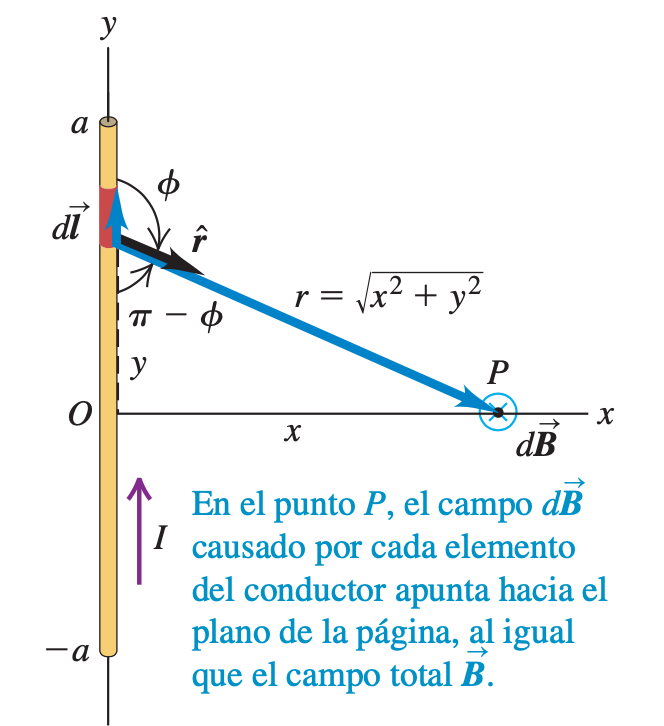
\includegraphics[scale=0.6]{fig/image1}
\caption{Campo magnético producido por un conductor recto portador de corriente de longitud infinita.}
\label{fig:28.5}
\end{figure}
Usando la ley de Biot y Savat, ecuación \ref{28.6}, y haciendo los cálculos correspondientes, se tiene que $B$ debe tener la misma magnitud en todos los puntos de un círculo con centro en el conductor y que yace en un plano perpendicular a él, y la dirección de $B$ debe ser tangente a todo ese círculo. Así, 
\begin{equation}\label{28.9}\marginnote{C. magnético cerca de un conductor largo y recto portador de corriente}
\boxed{\vec{B}=\frac{\mu_0I}{2\pi r}\hat{\phi}}
\end{equation}
\textbf{Observaciones:}
\begin{enumerate}
\item Las líneas de campo magnético circundan la corriente que actúa como su fuente.
\item Las líneas del campo magnético forman espiras cerradas y \textit{nunca} tienen extremos, sin importar la forma del conductor portador de corriente que genera el campo. Ésta es una consecuencia de la ley de Gauss para el magnetismo, que plantea que el flujo magnético total a través de cualquier superficie cerrada siem- pre es igual a cero:
\begin{equation}\label{28.10}
\oint\vec{B}\cdot d\vec{A}=0
\end{equation}
Esto implica que no hay cargas magnéticas aisladas ni monopolos magnéticos. \textbf{Cualquier línea de campo magnético que entre a una superficie cerrada debe salir de ella}.
\end{enumerate}
\section{Fuerza entre alambres paralelos}
\begin{figure}[h]\label{fig2}
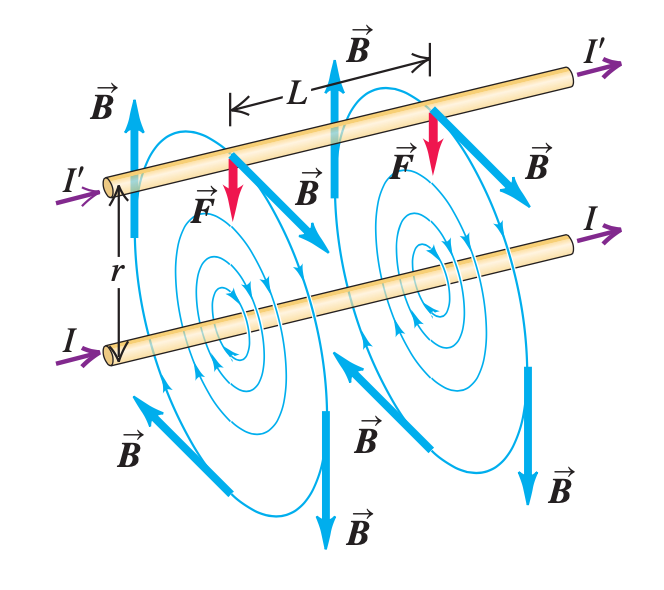
\includegraphics[scale=0.6]{fig/image2}
\centering
\end{figure}
De acuerdo con la ecuación \ref{28.9}, el conductor inferior produce un campo $\vec{B}$ que, en la posición del conductor de arriba, tiene una magnitud $$B=\frac{\mu_0I}{2\pi r}$$ De ecuación (27.19) la fuerza que ejerce este campo sobre una longitud $L$ del conductor superior es $\vec{F}=I' \vec{L}\times\vec{B}$,  donde el vector $\vec{L}$ está en dirección de la corriente $I'$ y tiene magnitud $L$. Como $\vec{B}$ es perpendicular a la longitud del conductor y, por lo tanto, a $\vec{L}$, la magnitud de esta fuerza es $$F=I'LB=\frac{\mu_oII'L}{2\pi r}$$ Luego, la \textit{fuerza por unidad de longitud}, $F/L$ está dada por
\begin{equation}\label{28.11}\marginnote{Magnitud de la fza. entre dos coductores largos, paralelos y portadores de
corriente}
\boxed{\frac{F}{L}=\frac{\mu_0II'}{2\pi r}}
\end{equation}
La aplicación de la regla de la mano derecha a $\vec{F}=I'\vec{L}\times\vec{B}$ indica que la fuerza sobre el conductor de arriba está dirigida hacia abajo.

\textbf{Observación}:
\begin{enumerate}
\item Dos conductores paralelos que transportan corrientes en el mismo sentido se atraen uno al otro.
\item Dos conductores paralelos que transportan corrientes en sentido opuestos se repelen entre sí.
\end{enumerate}
\section{Campo magnético de una espira circular de corriente}
\begin{figure}[h]\label{fig3}
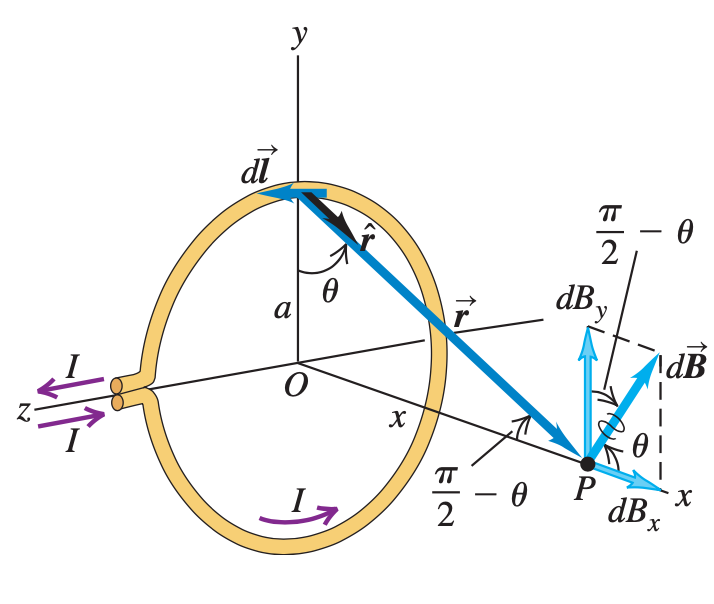
\includegraphics[scale=0.6]{fig/image3}
\centering
\end{figure}
Para encontrar el campo magnético en el punto $P$ sobre el eje de la espira, se usa la ley de Biot y Savart, ecuación \ref{28.5} o \ref{28.6}. De la figura \ref{fig3}, $d\vec{l}$ y $\vec{r}$ son perpendiculares, y la dirección del campo $d\vec{B}$ generado por este elemento $d\vec{l}$ en particular yace sobre el plano $xy$. La magnitud $dB$ del campo debido al elemento $d\vec{l}$ es
\begin{equation}\label{28.15}
\boxed{B_x=\frac{\mu_0Ia^2}{2(x^2+a^2)^{3/2}}}
\end{equation}
Si se cierran los dedos de la mano derecha alrededor de la espira en la dirección de la corriente, el pulgar derecho apunta en la dirección del campo.
\subsection{Campo magnético sobre el eje de una bobina}
Ahora suponga que en vez de una sola espira en la figura \ref{fig3}, se tiene una bobina que consiste en N espiras. Cada espira contribuye por igual al campo, y el total es N veces el campo producido por una sola espira:
\begin{equation}\label{28.16}
B_x=\frac{\mu_0NIa^2}{2(x^2+a^2)^{3/2}}
\end{equation}
En el centro de $N$ espiras circulares la magnitud del campo magnético vale
\begin{equation}\label{28.17}
\boxed{B_x=\frac{\mu_0Ia^2}{2a}}
\end{equation}
Conforme se avanza a lo largo del eje, la magnitud del campo disminuye.
\textbf{Observación}: Las ecuaciones \ref{28.15} y \ref{28.16} son válidas sólo sobre el \textit{eje} de una espira o bobina. No sobre otros puntos.


\section{Ley de Ampere}
\begin{equation}\label{28.20.ampere}\marginnote{Ley de Ampere}\footnote{Sólo válida si las corrientes son estables y si no están presentes materiales magnéticos o campos eléctricos que varíen con el tiempo.}
\boxed{\oint\vec{B}\cdot d\vec{l}=\mu_0I_{enc}}
\end{equation}
Hay una regla simple para determinar el signo de la corriente; Doble los dedos de su mano derecha alrededor de la trayectoria de integración en la dirección de esta última, es decir, la dirección que usa para evaluar $\oint\vec{B}\cdot d\vec{l}$. En esas condiciones, su pulgar derecho indica la dirección de la corriente positiva. Las corrientes que pasan a través de la trayectoria de integración en esta dirección son positivas; aquéllas en dirección opuesta son negativas. La ecuación \ref{28.20.ampere} de hecho es válida para conductores y trayectorias de \textbf{cualquier} forma.

\textbf{Observación}: Si $\oint\vec{B}\cdot d\vec{l}=0$, no necesariamente significa que $\vec{B}=0$
\subsection{Campo de un soleoide}
\begin{figure}[h]
\centering
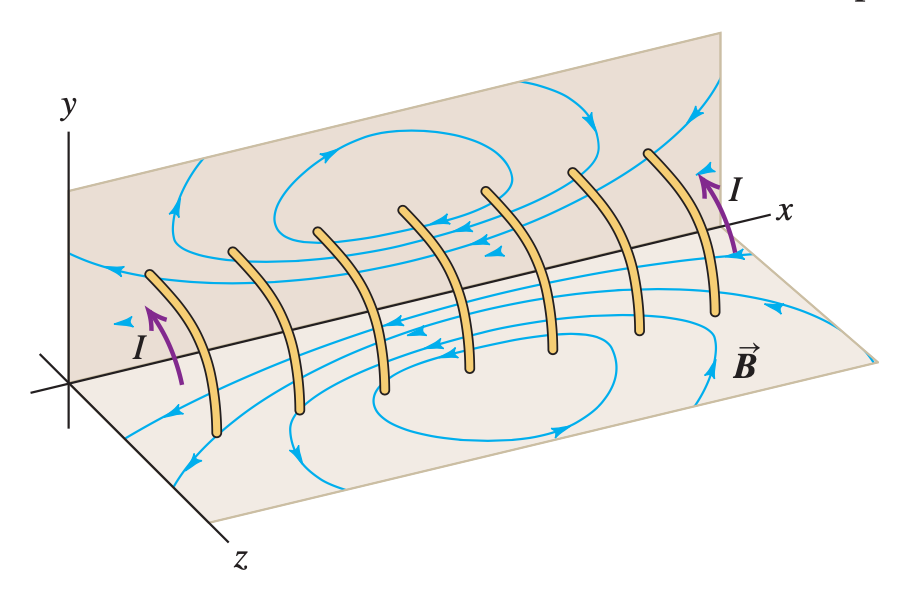
\includegraphics[scale=0.4]{fig/solenoide1}
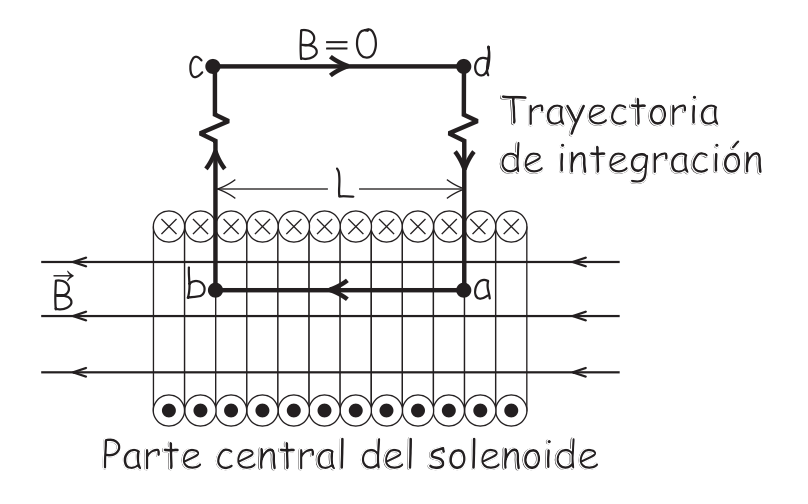
\includegraphics[scale=0.4]{fig/solenoide2}
\end{figure}
Aplicando la ley de Ampere, ecuación \ref{28.20.ampere}, junto con la trayectoria mostrada, se tiene que 
\begin{equation}
B=\mu_0nI
\end{equation}
teniendo en cuenta que $I_{enc}=nLI$.
\subsection{Campo de un solenoide toroidal(toroide)}
\begin{figure}[t]
\centering
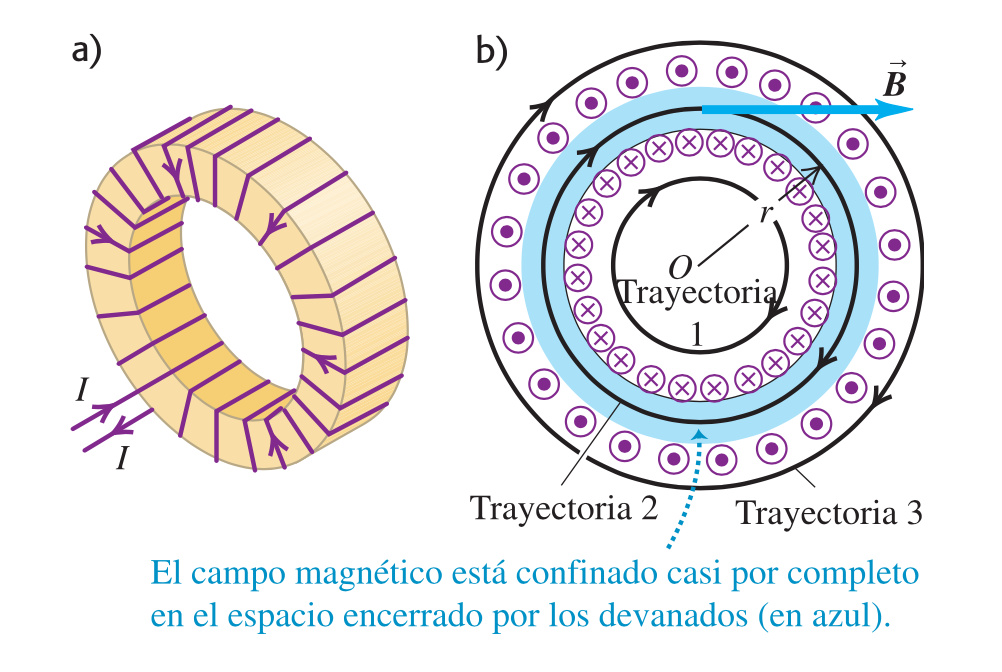
\includegraphics[scale=0.5]{fig/toroide}
\end{figure}
Considerando la trayectoria de integración 1. No hay corriente encerrada, luego $\vec{B}=0$ en cualquier punto de esta trayectoria.

Considernado la trayectoria de integración 3. Cada espira pasa dos veces a través del área limitada por esta trayectoria, llevando corrientes iguales en sentidos opuestos. Luego $I_{enc}=0\rightarrow \vec{B}=0$ en todos los puntos de esta trayectoria.

Considerando la trayectoria 2, un círculo con radio $r$. Se espera que el campo $\vec{B}$ sea tangente a la trayectoria. Por tanto, $\oint\vec{B}\cdot d\vec{l}=2\pi rB$. Despejando $B$
\begin{equation}\label{28.24.toroide}
B=\frac{\mu_0NI}{2\pi r}
\end{equation}
%\end{document}

\chapter{Inducción electromagnética}
La fuente de fem no es una batería, sino una estación generadora de electricidad.
La inducción electromagnética nos dice que un campo magnético que varía en el tiempo actúa como fuente de campo eléctrico.
También, un campo eléctrico que varía con el tiempo actúa como fuente de un campo magnético

\section{Ley de Faraday}
El flujo magnético total $\Phi_B$ a través de un área finita es la integral de esta expresión sobre el área:
\begin{equation}\label{29.1}
\Phi_B=\int\vec{B}\cdot d\vec{A}=\int B\, dA\cos\phi
\end{equation}
En el caso de que $\vec{B}$ sea uniforme sobre un área plana $\vec{A}$, entonces
\begin{equation}\label{29.2}
\Phi_B=\vec{B}\cdot \vec{A}=BA\cos\phi
\end{equation}
La \textbf{Ley de Faraday de la inducción} establece lo siguiente:
\textit{La fem inducida en una espira cerrada es igual al negativo de la tasa de cambio del flujo magnético a través de la espira con respecto al tiempo}.
 
En símbolos
\begin{equation}\marginnote{Ley de Faraday}\label{29.3.faraday}
\boxed{\varepsilon=-\frac{d\Phi_B}{dt}}
\end{equation}
\textbf{Obervación}: Las fem inducidas son ocasionadas por \textbf{cambios de flujo}.

Si se tiene una bobina con $N$ espiras idénticas y si el flujo varía a la misma tasa a través de cada espira, la fem total en la bobina es
\begin{equation}\label{29.4.Nfaraday}
\boxed{\varepsilon=-N\frac{d\Phi_B}{dt}}
\end{equation}
La \textbf{Ley de Lenz} establece que, \textit{la dirección de cualquier efecto de la inducción magnética es la que se opone a la causa del efecto.}
\section{Fuerza electromotriz de movimiento}
\begin{figure}[h]
\centering
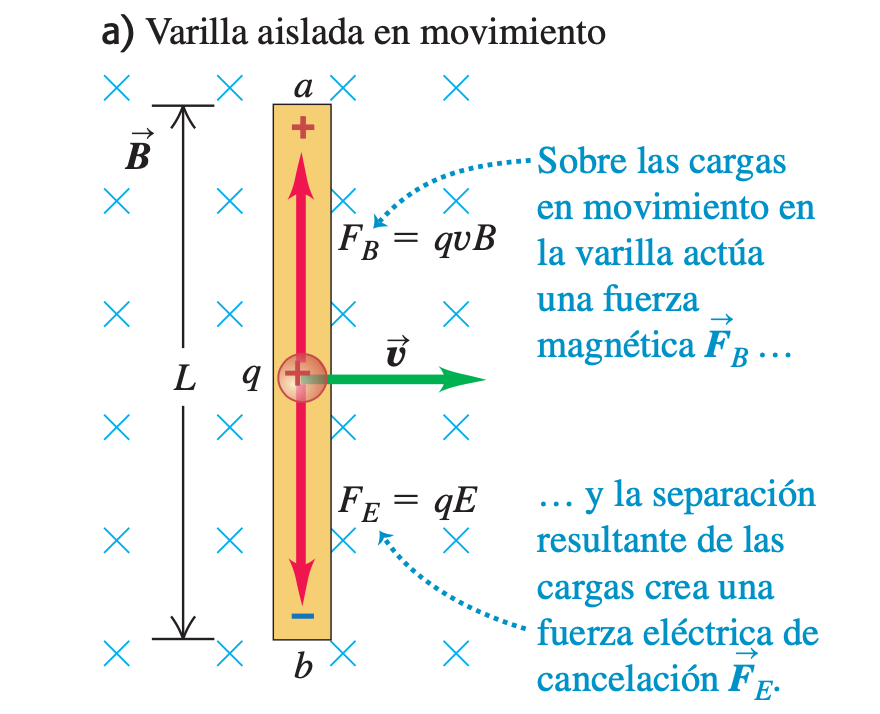
\includegraphics[scale=0.5]{fig/varilla}
\end{figure}
Una partícula cargada $q$ (	que suponemos positiva) en la varilla experimenta una fuerza magnética $\vec{F}=q\vec{v}\times\vec{B}$ con magnitud $F=|q|vB$. Esta fuerza magnética hace que las cargas libres en la varilla se muevan, lo que crea un exceso de carga positiva en el extremo superior $a$ y de carga negativa en el extremo inferior $b$.
Esto, a la vez, crea un campo eléctrico $\vec{E}$ en el interior de la varilla, en el sentido que va de $a$ hacia $b$ (opuesto al campo magnético). Llega un momento en el que $\vec{E}$ es lo suficientemente grande como para que la fuerza eléctrica ($qE$) cancele exáctamente a la magnética. De esta manera, $qE=qvB$, y las cargas están en equilibrio. Luego, se tiene que
\begin{equation}\label{29.5}
V_{ab}=V_a-V_b=EL=qBL
\end{equation}
con el punto $a$ a un potencial mayor que $b$.
\textbf{Continua...}
\subsection{Fem de movimiento: Forma general}
Podemos generalizar el concepto de fem de movimiento para un conductor de cualquier forma que se mueva en un campo magnético, uniforme o no (suponiendo que el campo magnético en cada punto no varía con el tiempo). Para cualquier fem cerrada, la fem total es
\begin{equation}\label{29.7}
\varepsilon=\oint (\vec{v}\times\vec{B})\cdot d\vec{l}
\end{equation}
Cuando se tienen conductores fijos en campos magnéticos cambiantes, no es posible utilizar la ecuación \ref{29.7}. En tal caso utilizar la ley de Faraday, ecuación \ref{29.3.faraday}.


\section{Campo eléctricos inducidos}
Una fem inducida también se presenta cuando hay un flujo cambiante a través de un conductor fijo.

\begin{figure}[h]\label{fig:galvanometro}
\centering
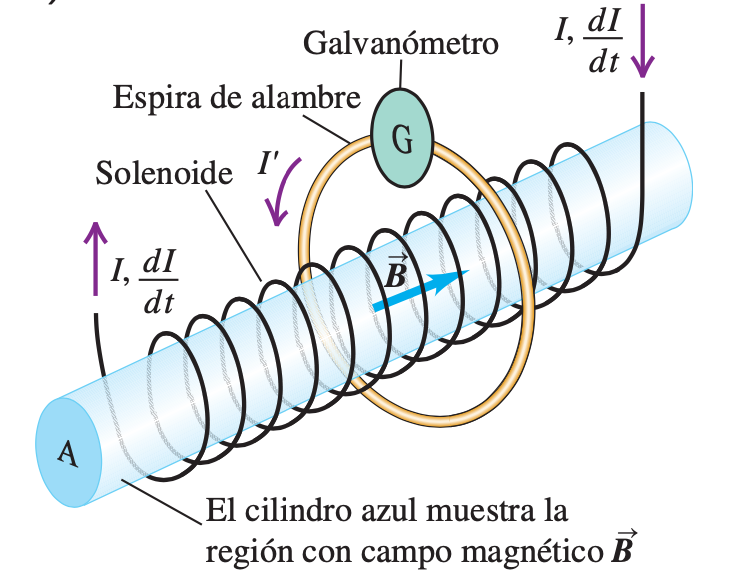
\includegraphics[scale=0.5]{fig/galvanometro}
\caption{El devanado de un solenoide largo lleva una corriente que se incrementa a una tasa $dI>dt$. El flujo magnético en el solenoide aumenta a una tasa $d\Phi_B/dt$, y este flujo cambiante pasa a través de una espira de alambre. En la espira se induce una fem $\varepsilon= -d\Phi_B/dt$, la cual induce una corriente $I'$ que se mide con el galvanómetro G}
\end{figure}

Consideremos la situacion que se ilustra en la figura \ref{fig:galvanometro}. Un solenoide largo y delgado, con área de sección transversal $A$ y $n$ espiras por unidad de
longitud, está rodeado en su centro por una espira conductora circular. El galvanómetro G mide la corriente en la espira. Una corriente $I$ en el devanado del solenoide establece un campo magnético $\vec{B}$ a lo largo de su eje, como se indica, con magnitud $B=\mu_0nI$, donde $n$ es el número de espiras por unidad de longitud. El flujo magnético a traves de la espira es $$\Phi_B=BA=\mu_0nIA$$ Cuando la corriente $I$ cambia con el tiempo se tiene, según la ley de Faraday

\begin{equation}\label{29.8}
\varepsilon=-\frac{d\Phi_B}{dt}=-\mu_0nA\frac{dI}{dt}
\end{equation}

Si la resistencia total de la espira es $R$, la corriente inducida en la espira es $I'=\varepsilon/R$. ¿Qué fuerza hace que las cargas se muevan alrededor de la espira? No puede ser una fuerza magnética porque el conductor no se está moviendo en un campo magnético, y en realidad ni siquiera está en un campo magnético. Se debe a un \textbf{campo magnético inducido} en el conductor \textit{causado por el flujo magnético cambiante}. Este campo eléctrico en la espira \textbf{no es conservativo}, porque la integral de línea de $\vec{E}$ a lo largo de la trayectoria cerrada no es igual a cero. En vez de ello, esta integral de línea, que representa el trabajo realizado por el campo inducido $\vec{E}$ por unidad de carga, es igual a la fem inducida $\varepsilon$:

\begin{equation}\label{29.9}
\oint\vec{E}\cdot d\vec{l}=\varepsilon
\end{equation}

Que según la ley de Faraday

\begin{equation}\label{29.10}\marginnote{Trayectoria de integración constante}
\boxed{\oint\vec{E}\cdot d\vec{l}=-\frac{d\Phi_B}{dt}}
\end{equation}

La forma de la ley de Faraday dada en la ecuación \ref{29.10}, sólo es válida si la trayectoria alrededor de la cual se integra es \textbf{constante}.

Un campo de esta clase recibe el nombre de \textbf{campo no electrostático}. Este campo, a pesar de no ser conservativo, ejerce una fuerza $\vec{F}=q\vec{E}$ sobre una carga $q$. De esta manera, un campo magnético actúa como fuente de campo eléctrico de una clase que \textit{no podemos} producir con ninguna distribución de carga estática.

\section{Corriente de desplazamiento y ecuaciones de Maxwell}
De igual manera que un campo magnético que varía da lugar a un campo eléctrico inducido, un campo eléctrico variable, da lugar a un campo magnético.

\subsubsection{Generalización de la ley de Ampere}
Recordando la ley de Ampere, $$\oint\vec{B}\cdot d\vec{l}=\mu_0I_{enc}$$ Esta ley, expresada de esta manera está \textit{incompleta}.
\textbf{continua...}







%\end{document}

\chapter{Inductancia}
\section{Inductancia mutua}

\begin{figure}[h]
\centering
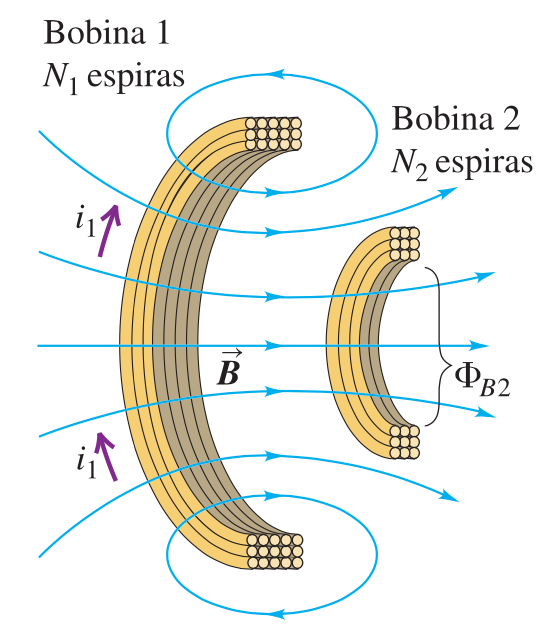
\includegraphics[scale=0.3]{fig/bobinas}
\caption{\textbf{Inductancia mutua}, si la corriente en la bobina 1 está cambiando, el flujo cambiante a través de la bobina 2 indice una fem en esta última}
\label{fig:bobinas}
\end{figure}
Interacción magnética entre dos alambres que trasnportan corrientes \textit{estables}; la corriente de uno de los alambres genera un campo magnético que ejerce una fuerza sobre la corriente entre el otro alambre. Cuando hay una corriente \textit{variable} en uno de los circuitos, surge una interacción adicional. Consideremos la situación de la figura
\ref{fig:bobinas}

Una corriente que circula por la bobina 1 produce un campo magnético $\vec{B}$ y, por lo tanto, un flujo magnético a través de la bobina 2. Si la corriente en la bobina 1 cambia, el flujo a través de la bobina 2 también cambia; de acuerdo con la ley de Faraday, esto induce una fem en la bobina 2. De este modo, un cambio en la corriente de un circuito puede inducir otra corriente en un segundo circuito.
Una corriente $i_1$\footnote{Denotamos con $i$ a una corriente variable en el tiempo } establece un campo magnético (indicado por las líneas de color azul), y algunas de estas líneas de campo pasan a través de la bobina 2. Denotaremos con $\Phi_{B2}$ el flujo magnético a través de \textit{cada} espira de la bobina 2, causado por la corriente $i_1$ en la bobina 1. (Si el flujo es diferente a través de las distintas espiras de la bobina, entonces $\Phi_{B2}$ denota el flujo  \textit{medio}). El campo magnético es proporcional a $i_1$, de manera que $\Phi_{B2}$ también es proporcional a $i_1$. \textbf{Cuando $i_1$ cambia, $\Phi_{B2}$ cambia; este flujo cambiante induce una fem $\varepsilon_2$ en la bobina 2}, dada por
\begin{equation}\label{fem}
\varepsilon_2=-N_2\frac{d\Phi_{B2}}{dt}
\end{equation}
Podríamos representar la proporcionalidad entre $\Phi_{B2}$ e $i_1$ en la forma $\Phi_{B2}$ = (constante) $i_1$, pero, en vez de ello, es más conveniente incluir el número de espiras $N_2$ en la relación. Al introducir una constante de proporcionalidad $M_{21}$, llamada \textbf{inductancia mutua} de las dos bobinas, escribimos
\begin{equation}\label{30.2}
N_2\Phi_{B2}=M_{21}i_1
\end{equation}
donde $\Phi_{B2}$ es el flujo a través de una sola espira de la bobina 2. De ahí que,
\begin{equation}
N_2\frac{d\Phi_{B2}}{dt}=M_{21}\frac{di_1}{dt}
\end{equation}
y la ecuación \ref{fem} se rescribe como
\begin{equation}
\varepsilon_2=-M_2\frac{di_1}{dt}
\end{equation}
Es decir, un cambio en la corriente $i_1$ en la bobina 1 induce una fem en la bobina 2, que es directamente proporcional a la tasa de cambio de $i_1$.

También se podría escribir la definición de la inductancia mutua, ecuación \ref{30.2}, como
\begin{equation}
M_{21}=\frac{N_2\Phi_{B2}}{i_1}
\end{equation}
\textbf{Si las bobinas están en el vacío}, el flujo $\Phi_{B2}$ a través de cada espira de la bobina 2 es directamente proporcional a la corriente $i_1$. Entonces, la inductancia mutua $M_{21}$ es una constante que sólo depende de la geometría de las dos bobinas.
Podría volverse a hacer el análisis para el caso opuesto, en el que una corriente cambiante $i_2$ en la bobina 2 causa un flujo cambiante $\Phi_{B}2$ y una fem $\varepsilon_1$ en la bobina 1. Se encuentra que, \textbf{$M_{12}$ siempre es igual a $M_{21}$, aun cuando las dos bobinas no sean simétricas}. A este valor común $M$ lo llamamos simplemente \textbf{inductancia mutua}. Por tanto, tenemos:
\begin{equation}\marginnote{Fem mutuamente inducidas}
\boxed{\varepsilon_2=-M\frac{di_1}{dt}\quad\mathrm{y}\quad \varepsilon_1=-M\frac{di_2}{dt}\quad}
\end{equation}
donde la inductancia mutua $M$ es
\begin{equation}\marginnote{Inductancia mutua}
\boxed{M=\frac{N_2\Phi_{B2}}{i_1}=\frac{N_1\Phi_{B1}}{i_2}}
\end{equation}
\textbf{Obs: Sólo una corriente variable en el tiempo induce una fem}.

La unidad del SI para la inductancia mutua se llama \textbf{henry} [$H$]
\section{Autoinductancia a inductores}
\begin{figure}[h]\label{fig:autoinductancia}
\centering
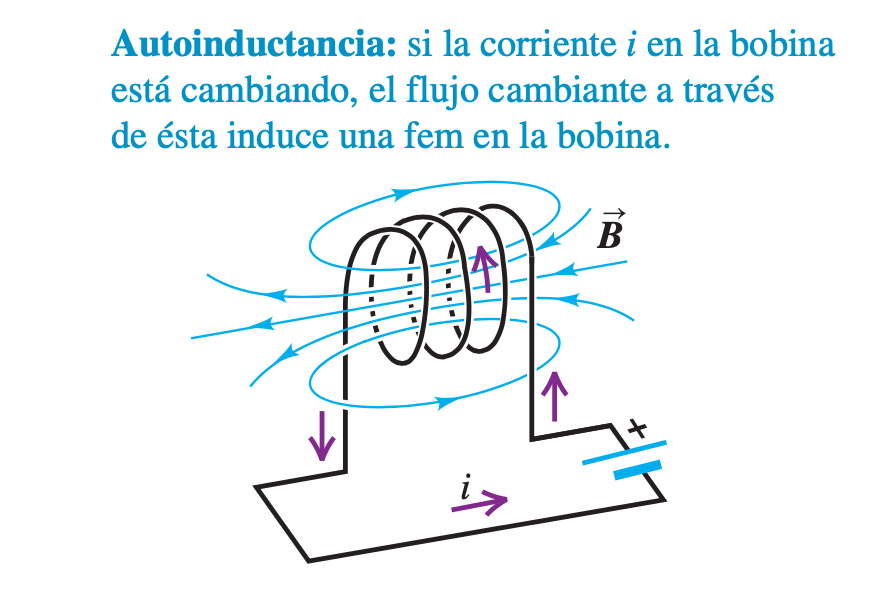
\includegraphics[scale=0.4]{fig/autoinductancia}
\caption{La corriente $i$ en el circuito crea un campo magnético $\vec{B}$ en la bobina y, por lo tanto, un flujo a través de ésta.}
\end{figure}

Consideremos un solo circuito aislado. Cuando en el circuito está presente una corriente, se establece un campo magnético que crea un flujo magnético a través del mismo circuito; este flujo cambia cuando la corriente cambia. Así, cualquier circuito que conduzca una corriente variable tiene una fem inducida en él por la variación en su propio campo magnético. Esa clase de fem se denomina \textbf{fem autoinducida}. Según la ley de Lenz, una fem autoinducida siempre se opone al cambio en la corriente que causó la fem, y de ese modo hace más difícil que haya variaciones en la corriente. El efecto se intensifica considerablemente si el circuito incluye una bobina con $N$ espiras de alambre. Como resultado de la corriente $i$, hay un flujo magnético medio $\Phi_B$ a través de cada vuelta de la bobina, figura \ref{fig:autoinductancia}.

Definimos la \textbf{autoinductancia} como
\begin{equation}\label{30.6.autoinductancia}\marginnote{Autoinductancia}
\boxed{L=\frac{N\Phi_B}{i}}
\end{equation}
Si la corriente $i$ en el circuito cambia, también lo hace el flujo $\Phi_B$. De ecuación \ref{30.6.autoinductancia} $$N\frac{d\Phi_B}{dt}=L\frac{di}{dt}$$ Utilizando la ley de Faraday, ecuación \ref{29.4.Nfaraday}, la fem autoinducida es
\begin{equation}\label{30.7}\marginnote{Fem autoinducida}
\boxed{\varepsilon=-L\frac{di}{dt}}
\end{equation}

\subsection{Los inductores como elementos de un circuito}
Un elemento de circuito diseñado para tener una inductancia particular se llama \textbf{inductor, o bobina de autoinducción}. Su finalidad es oponerse a cualquier variación en la corriente a través del circuito. Un inductor en un circuito de corriente directa ayuda a mantener una corriente estable a pesar de las fluctuaciones en la fem aplicada; en un circuito de corriente alterna, un inductor tiende a suprimir las variaciones de la corriente que ocurran más rápido de lo deseado.

Al utilizar la ley de Kirchhoff a traves de una malla conductora se suman sus diferencias de potencial y se igualan a cero porque el campo eléctrico producido por las cargas distribuidas es \textit{conservativo} ($\vec{E_c}$). El campo eléctrico inducido magnéticamente dentro de las bobinas del inductor \textbf{no es conservativo} ($\vec{E_n}$).


\begin{figure}[h]\label{fig30.5.circuito}
\centering
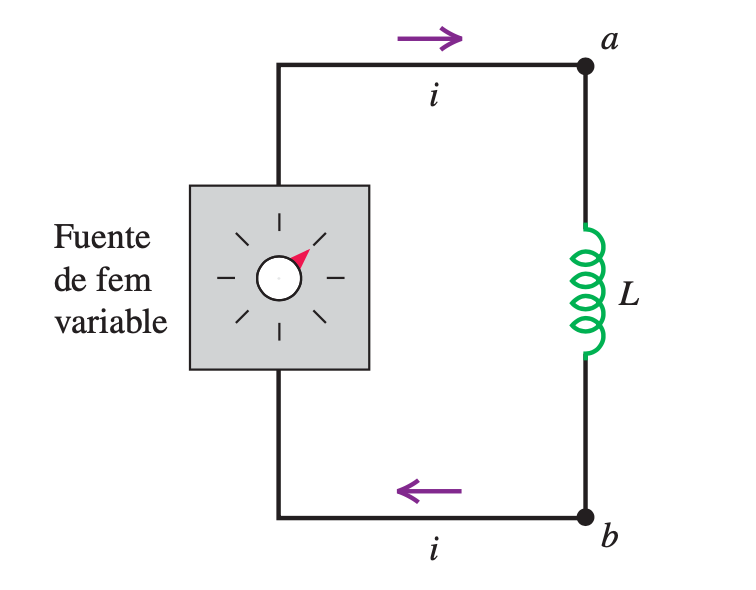
\includegraphics[scale=0.4]{fig/circuito}
\caption{Circuito que contiene una fuente de fem y un inductor. La fuente es variable, por lo que la corriente $i$ y su tasa de cambio $di>dt$ pueden variarse.}
\end{figure}

Consideremos el circuito de la figura \ref{fig30.5.circuito}. De acuerdo con la ley de Faraday, ecuación \ref{29.10}, la integral de línea de $\vec{E_n}$ alrededor del circuito es el negativo de la tasa de cambio del flujo a través del circuito. De ecuación \ref{30.7} $$\oint\vec{E_n}\cdot d\vec{l}=-L\frac{di}{dt}$$ donde se integra en sentido horario del circuito (el sentido supuesto para la corriente). Pero $\vec{E_n}$ es diferente de cero sólo dentro del inductor. Entonces $$\int_a^b\vec{E_n}\cdot d\vec{l}=-L\frac{di}{dt}$$ A continuación, como $\vec{E_c}+\vec{E_n}=0$ en cada punto dentro de las bobinas del inductor $$\int_a^b\vec{E_c}\cdot d\vec{l}=L\frac{di}{dt}$$ Pero esta integral es el potencial $V_{ab}$ del punto $a$ con respecto a $b$

\begin{equation}\label{30.8}
V_{ab}=V_a-V_b=L\frac{di}{dt}
\end{equation}

Se concluye que hay una diferencia de potencial genuina entre las terminales del inductor, asociada con las fuerzas conservativas electrostáticas, a pesar del hecho de que el campo eléctrico asociado con el efecto de inducción magnética es no conservativo.
\textbf{Obervación}: La fem autoinducida se opone a los cambios de la corriente ($di/dt$), \textit{no} a la corriente $i$ en sí.

\section{Energía del campo magnético}
El establecimiento de una corriente en un inductor requiere un suministro de energía, y un inductor que conduce corriente contiene energía almacenada. En la figura \ref{fig30.5.circuito}, una \textit{corriente creciente} $i$ ($di/dt>0$) en el inductor produce una fem $\varepsilon$ entre sus terminales, y una diferencia de potencial correspondiente $V_{ab}$ entre las terminales de la fuente, con el punto $a$ a mayor potencial que el $b$. Así, la fuente debe estar agregando energía al inductor, y la potencia instantánea $P$ (la tasa de transferencia de energía al inductor) es $P=V_{ab}i$.

\subsubsection{Energía almacenada en un inductor}
Si la corriente inicial es igual a cero, con la inductancia $L$ podemos calcular la entrada total de energía $U$ necesaria para establecer una corriente final $I$ en un inductor. Suponemos que el inductor tiene una resistencia igual a cero, por lo que dentro del inductor no se disipa energía. El voltaje entre las terminales $a$ y $b$ del inductor en ese instante es $V_{ab}=L\frac{di}{dt}$, y la tasa $P$ a la que se entrega energía al indutor (igual a la potencia instantánea suministrada por la fuente) es

\begin{equation*}
P=V_{ab}i=L\frac{di}{dt}
\end{equation*}

La energía $dU$ suministrada al inductor durante un intervalo de tiempo infinitesimal $dt$ es $dU=Pdt$, por lo que

\begin{equation*}
dU=Lidi
\end{equation*}

La energía total $U$ suministrada mientras la corriente aumenta de cero a un valor final
$I$ es

\begin{equation}\label{30.9}\marginnote{Energía almacenada en un inductor}
\boxed{U=L\int_0^{I}i\, dt=\frac{1}{2}LI^2}
\end{equation}

Una vez que la corriente ha alcanzado su valor final estable $I$, $di/dt=0$, y no se alimenta más energía al inductor. Cuando no hay corriente, la energía almacenada $U$ es igual a cero; cuando la corriente es $I$, la energía es $\frac{1}{2}LI^2$.

Cuando la corriente disminuye de $I$ a cero, el inductor actúa como fuente que suministra una cantidad total de energía igual a $\frac{1}{2}LI^2$ al circuito externo. Si interrumpimos bruscamente el circuito abriendo un interruptor o desconectando violentamente una clavija (enchufe) de una toma de corriente de pared, la corriente disminuye con mucha rapidez, la fem inducida es muy grande y la energía podría disiparse en forma de un arco entre los contactos del interruptor.

\textbf{Observación:} Es importante no confundir el comportamiento de resistores e inductores en lo que respecta a la energía. La energía fluye hacia un resistor siempre que una corriente, ya sea estable o variable, pasa a través de él; esta energía se disipa en forma de calor. En contraste, la energía fluye hacia un inductor ideal con resistencia igual a cero, sólo cuando la corriente en este último se \textit{incrementa}. Esta energía no se disipa, sino que se almacena en el inductor y se libera cuando la corriente \textit{disminuye}. Cuando una corriente estable fluye a través de un inductor, no entra ni sale energía

\subsubsection{Densidad de la energía magnética}
La energía en un inductor en realidad se almacena en el campo magnético dentro de la bobina, al igual que la energía de un capacitor lo hace en el campo eléctrico entre sus placas. Nos centraremos en un caso sencillo: el del solenoide toroidal ideal. Su campo magnético se encuentra confinado por completo en una región finita del espacio en el interior de su núcleo. La inductancia del selenoide toroidal con vacío dentro de sus bobinas es 

\begin{equation}\label{L de un toroide}\marginnote{Inductancia de un toroide}
L=\frac{\mu_0N^2A}{2\pi r}
\end{equation}

De ecuación \ref{30.9}, la energía $U$ alamacenada en el toroide  cuando la corriente es $I$ es

\begin{equation*}
U=\frac{1}{2}LI^2=\frac{1}{2}\frac{\mu_0N^2A}{2\pi r}I^2
\end{equation*}

El campo magnético y, por lo tanto, esta energía se localizan en el volumen $V=2\pi rA$ encerrado por los devanados. La energía por \textit{unidad de volumen}, o \textit{densidad de energía magnética}, es $u=U/V$:

\begin{equation}\label{u}
u=\frac{U}{2\pi rA}=\frac{1}{2}\mu_0\frac{N^2I^2}{(2\pi r)^2}
\end{equation}

Expresandola en términos de la magnitud $B=(\mu_0NI)/(2\pi r)$ del campo magnético dentro del toroide es

\begin{equation*}
\frac{N^2I^2}{(2\pi r)^2}=\frac{B^2}{\mu_0^2}
\end{equation*}

Sustituyendo esto en \ref{u}, se encuentra que la expresión para la \textbf{densidad de energía magnética} en el vacío es

\begin{equation}\label{30.10.u}\marginnote{Densidad de energía magnética en el vacío}
\boxed{u=\frac{B^2}{2\mu_0}}
\end{equation}

Cuando el material dentro del toroide no es un vacío, sino un material con permeabilidad magnética (constante) $\mu=K_m\mu_0$, se sustituye $\mu_0$ por $\mu_0$ en la ecuación \ref{30.10.u}. Así, la energía por unidad de volúmen en el campo magnético es

\begin{equation}\label{30.11.u2}\marginnote{Densidad de energía magnética en un material}
\boxed{u=\frac{B^2}{2\mu}}
\end{equation}

La expresión \ref{30.11.u2} resulta ser correcta para \textit{cualquier} configuración de campo magnético en un material con permeabilidad constante. 

\section{El circuito R-L}
Un inductor en un circuito hace difícil que ocurran cambios rápidos en la corriente, en virtud de los efectos de la fem autoinducida. La ecuación \ref{30.7} muestra que cuanto más grande es la tasa de cambio de la corriente, $di/dt$, mayor es la fem autoinducida y mayor la diferencia de potencial entre las terminales del inductor.

\subsection{Crecimiento de la corriente en un circuito R-L}

\begin{figure}[b]\label{fig:circuito2}
\centering
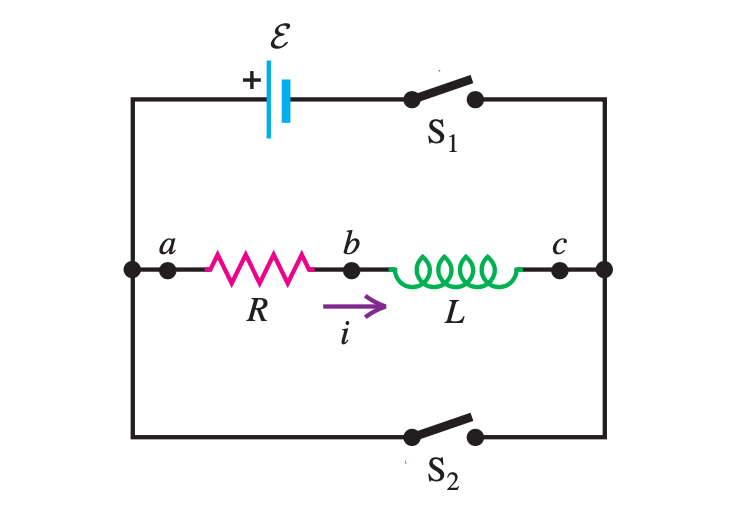
\includegraphics[scale=0.4]{fig/circuito2}
\caption{Al cerrar el interruptor $S_1$ se conecta la combinación $R-L $en serie con una fuente de fem $\varepsilon$. Al cerrar el interruptor $S_2$ al mismo tiempo que se abre $S_1$ se desconecta la combinación de la fuente.}
\end{figure}

Un circuito que incluye tanto un resistor como un inductor, y tal vez una fuente de fem, se llama circuito $R_L$ (figura \ref{fig:circuito2}).  El inductor ayuda a impedir los cambios rápidos en una corriente, lo que puede ser útil si se requiere una corriente estable y la fuente externa tiene una fem fluctuante.







%\end{document}

\end{document}

